\section[Problem 2]{Problem 2: Gated SAR--Optical Fusion with Area Calibration and Probabilistic Grading}
\label{sec:q2}

\subsection{Inherited Settings and New Components}

Nothing in Problem~2 starts from zero. The preprocessing, the folds \eqref{eq:folds}, the metrics \eqref{eq:area_metrics} and the land-cover strata carry over from Problem~1 unchanged; every number below can be read against Table~\ref{tab:q1_metrics} on the same 1000 held-out tiles (all variants share one test-tile hash). What changes answers the four diagnoses of Section~\ref{sec:q1}, one component each. Fragmented flood and isolated dark surfaces need spatial context, which a pixel classifier does not have; the classifier gives way to a convolutional network. Dark fields and permanent ponds need the pre-flood optical state, which enters through gated feature fusion. An area-aware loss during training, followed by an area calibration, answers the positive total bias. Tile-level intervals carry the uncertainty into the grading, where it has to survive the transfer. Hengzhou adds a fifth requirement no component above provides: the model must run when the optical input is missing.

\subsection{Dual-Branch Gated Fusion Network}

Two U-Net encoders~\cite{ronneberger2015unet} form the network. The SAR branch reads $[z,\tilde z,\mathrm{std}_7(\tilde z)]$; the optical branch reads $[B,G,R,N]/255$, NDWI, NDVI and the validity $m_p$. Four stages of width 16, 32, 64 and 128 make up each branch (two $3\times3$ convolutions with batch normalization and ReLU, then $2\times2$ max-pooling). At every scale $s$ a learned gate mixes the two feature maps $h_S^{(s)}$ and $h_O^{(s)}$,
\begin{equation}
g^{(s)}=\sigma\!\left(W_g^{(s)}*\big[h_S^{(s)};h_O^{(s)}\big]\right),\qquad
h^{(s)}=g^{(s)}\odot h_S^{(s)}+\big(1-g^{(s)}\big)\odot h_O^{(s)},
\label{eq:gate}
\end{equation}
where $W_g^{(s)}$ is a $1\times1$ convolution, $\sigma$ the logistic function and $\odot$ the element-wise product. The fused map feeds the skip connection of a U-Net decoder (bottleneck 256 channels, bilinear upsampling, dropout 0.2), which ends in a $1\times1$ convolution to the logit $o_p$. Parameters number 2.30\,M, and Fig.~\ref{fig:arch_fusion} shows the data flow.

\begin{figure}[!ht]
  \centering
  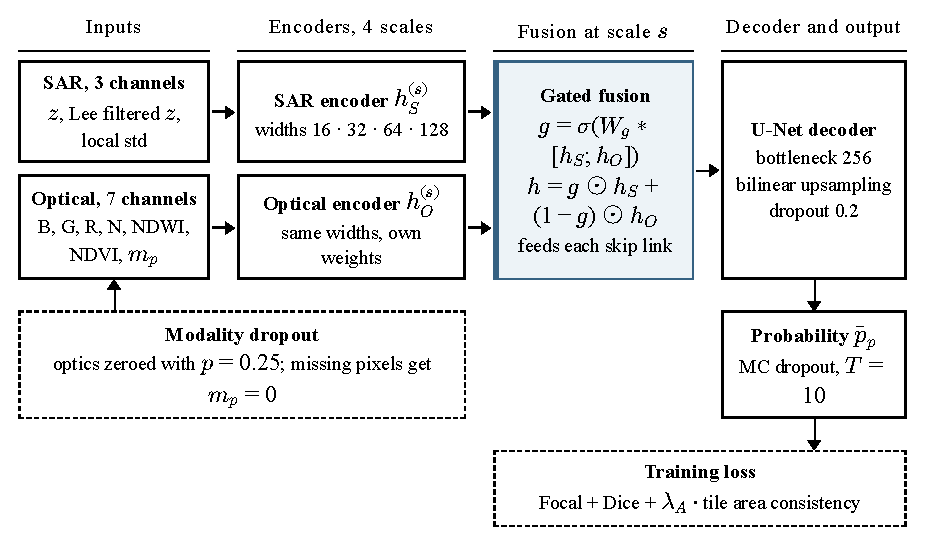
\includegraphics[width=0.90\textwidth,keepaspectratio]{../figures/fig_arch_fusion.pdf}
  \caption{Dual-branch gated fusion network}
  \label{fig:arch_fusion}
\end{figure}

Per pixel and per channel, the gate of \eqref{eq:gate} decides how much to trust each sensor. Where the optical image says ``river before the flood'', the gate can lean on optics to suppress a SAR-dark pixel; where optics are cloudy, it can lean on SAR. Weight is distributed almost evenly: mean SAR gate values are 0.52, 0.57, 0.56 and 0.53 at the four scales, and neither sensor is ignored. A modality-dropout block at the bottom of Fig.~\ref{fig:arch_fusion} sets the entire optical input and $m_p$ to zero with probability 0.25 per training sample, and invalid optical pixels are always zeroed. Working from SAR alone where optics are missing is part of what the model learns; Hengzhou is exactly that case (Section~\ref{sec:q3}).

\textbf{Area-consistent loss.} With $\hat p_p=\sigma(o_p)$, $\hat p_{p,y}$ the probability of the true class, batch $\mathcal B$ and $N_b$ valid pixels in sample $b$, training minimizes
\begin{equation}
\mathcal L=-\frac{1}{|\mathcal V|}\sum_p\alpha_y(1-\hat p_{p,y})^{\gamma}\log\hat p_{p,y}
+\left(1-\frac{2\sum_p\hat p_py_p+1}{\sum_p\hat p_p+\sum_py_p+1}\right)
+\frac{\lambda_A}{|\mathcal B|}\sum_{b\in\mathcal B}\frac{\big|\sum_{p\in b}(\hat p_p-y_p)\big|}{N_b},
\label{eq:loss}
\end{equation}
a focal term~\cite{lin2017focal} ($\gamma=2$, $\alpha_1=0.75$) against the imbalance, a Dice term against the dominance of empty pixels, and an area-consistency term that penalizes the difference between the expected and the true flood area of each tile. Training uses Adam with learning rate $10^{-3}$ and cosine decay, batch 16, flips and $90^\circ$ rotations, at most 40 epochs, and early stopping on the calibration-fold MAE$_A$ with patience 8.

\subsection{Turning Probabilities into an Unbiased Area}

A segmentation threshold of 0.5 maximizes neither accuracy nor area agreement. We therefore calibrate on the calibration fold in three steps.

\textbf{(i) Ensemble mean.} With dropout active at inference, $T=10$ stochastic forward passes give $\bar p_p=\frac1T\sum_{\ell}\hat p_p^{(\ell)}$.

\textbf{(ii) Isotonic calibration.} A monotone map $q$ estimates $\Pr(y=1\mid\bar p)$~\cite{zadrozny2002calibration}:
\begin{equation}
q=\arg\min_{q\ \text{non-decreasing}}\ \sum_{p\in\mathrm{cal}}\big(y_p-q(\bar p_p)\big)^2 .
\label{eq:isotonic}
\end{equation}

\textbf{(iii) Area-preserving threshold.} $\tau_A$ is chosen so that the area of the binary mask equals the calibrated expected area:
\begin{equation}
\sum_{p\in\mathrm{cal}}a_p\,\mathbb 1\big[\bar p_p\ge\tau_A\big]=\sum_{p\in\mathrm{cal}}a_p\,q(\bar p_p).
\label{eq:tauA}
\end{equation}
The left side is non-increasing in $\tau_A$, the right side is constant, and bisection on $[0.01,0.99]$ with tolerance $10^{-4}$ finds the solution. The final mask is $\hat F=\{\bar p\ge\tau_A\}$, and the reported area is the area of that mask; maps and areas agree by construction. Fold thresholds were $\tau_A=0.708$, 0.515, 0.388, 0.690 and 0.574. Calibration folds give a mask area of 933.111\,km$^2$ against an expected 933.112\,km$^2$, a relative gap of $6\times10^{-7}$. On calibration data the identity holds exactly; on test data the remaining bias is an empirical result.

\textbf{Tile intervals.} The MC spread of the tile area, $\sigma_t=\mathrm{std}_\ell\big(\sum_{p\in t}a_p\mathbb 1[\hat p^{(\ell)}_p\ge\tau_A]\big)$, is stabilized as $\sigma'_t=\sigma_t+c$ with $c$ the larger of the calibration median of $\sigma_t$ and 0.005\,km$^2$. Split-conformal prediction~\cite{lei2018conformal} then gives a distribution-free tile interval:
\begin{equation}
\begin{split}
s_t&=\frac{|A_t-\hat A_t|}{\sigma'_t},\qquad
\hat q=s_{(\lceil(n+1)(1-\alpha)\rceil)},\\
\mathcal I_t&=\Big[\max(0,\ \hat A_t-\hat q\sigma'_t),\ \min(A^{tile}_t,\ \hat A_t+\hat q\sigma'_t)\Big],
\end{split}
\label{eq:conformal}
\end{equation}
with $\alpha=0.1$, scores $s_t$ from the $n\approx200$ calibration tiles of the fold, and $A^{tile}_t$ the tile area. The signed standardized residuals $r_t=(A_t-\hat A_t)/\sigma'_t$ of all calibration folds form the residual pool $\mathcal R$ used for the grade uncertainty below.

\subsection{Ablation: Which Component Reduces the Area Error}

Seven trained variants share a held-out set: M0 is the Problem~1 LightGBM; M1 a SAR-only U-Net (focal and Dice loss); M2 adds the gated optical branch; M3 an area term ($\lambda_A=1$); M4 modality dropout and the validity channel; M5 the MC-dropout mean; M6 isotonic calibration and $\tau_A$. The two MMU rows apply 50 px post-processing to M2 and M6 and are not ablation steps. Table~\ref{tab:q2_ablation} lists the metrics.

\begin{table}[!ht]
\centering
\caption{Ablation on all and hard held-out tiles}
\label{tab:q2_ablation}
\resizebox{\textwidth}{!}{%
\begin{tabular}{lcccccccc}
\toprule
 & \multicolumn{6}{c}{All 1000 tiles} & \multicolumn{2}{c}{397 hard tiles} \\
\cmidrule(lr){2-7}\cmidrule(lr){8-9}
Variant & IoU & F1 & $\kappa$ & RAE & MAE$_A$ (km$^2$) & median $|\mathrm{RAE}_t|$ & IoU & RAE \\
\midrule
A physics baseline & 0.278 & 0.435 & 0.227 & $+1.406$ & 1.756 & 2.84 & -- & -- \\
M0 LightGBM & 0.598 & 0.749 & 0.686 & $+0.092$ & 0.430 & 0.52 & 0.266 & $+0.208$ \\
M1 U-Net, SAR only & 0.549 & 0.709 & 0.628 & $+0.349$ & 0.509 & 0.50 & 0.420 & $+0.433$ \\
M2 + gated optical fusion & 0.798 & 0.888 & 0.861 & $+0.034$ & 0.149 & 0.17 & 0.649 & $+0.035$ \\
M2 + 50 px MMU & 0.797 & 0.887 & 0.860 & $+0.009$ & 0.150 & 0.20 & 0.648 & $-0.020$ \\
M3 + area loss & 0.793 & 0.885 & 0.857 & $+0.034$ & 0.160 & 0.20 & 0.664 & $+0.044$ \\
M4 + modality dropout & 0.737 & 0.849 & 0.812 & $+0.041$ & 0.227 & 0.30 & 0.575 & $+0.010$ \\
M5 + MC-dropout mean & 0.737 & 0.849 & 0.812 & $+0.039$ & 0.227 & 0.31 & 0.575 & $+0.002$ \\
M6 + isotonic and $\tau_A$ & 0.732 & 0.845 & 0.808 & $+0.0145$ & 0.236 & 0.31 & 0.562 & $-0.052$ \\
M6 + 50 px MMU & 0.730 & 0.844 & 0.807 & $0.000$ & 0.238 & 0.35 & 0.558 & $-0.085$ \\
\bottomrule
\end{tabular}}
\end{table}

No single variant wins every metric. Optical fusion leads IoU (0.798) and F1 (0.888); in the hard block M3 has the highest IoU (0.664) and M6+MMU the smallest RAE ($-0.085$). The MMU acts on area only: it takes M2's all-tile RAE from 3.4\% to 0.9\% and its hard-set bias from $+3.5\%$ to $-2.0\%$, and M2+MMU is the only row with a total RAE below 1\%.

Pixel overlap and area calibration are different objectives: M6+MMU reaches a total bias of $0.0\%$ yet loses 6.7 pp IoU and 9.0 pp hard-set IoU against M2+MMU, so calibration repairs the area of a weaker backbone, not its pixel accuracy. M2 leads MAE$_A$ (0.149\,km$^2$); its MMU removes 1.3\% of true positives and 10.3\% of false positives. The largest relative change is in the hard columns: on the 397 tiles where LightGBM had $|\mathrm{RAE}_t|>0.5$, M2+MMU lifts IoU from 0.266 to 0.648 (M6: 0.562), cuts MAE$_A$ from 0.620 to 0.163\,km$^2$ and moves RAE from $+20.8\%$ to $-2.0\%$.

Fig.~\ref{fig:q2_ablation} isolates each step: the change of IoU, MAE$_A$ and $|\mathrm{RAE}|$ attributed to the component added there (LightGBM dashed), open dots before and filled dots after, green and red for improvement and degradation.

\begin{figure}[!ht]
  \centering
  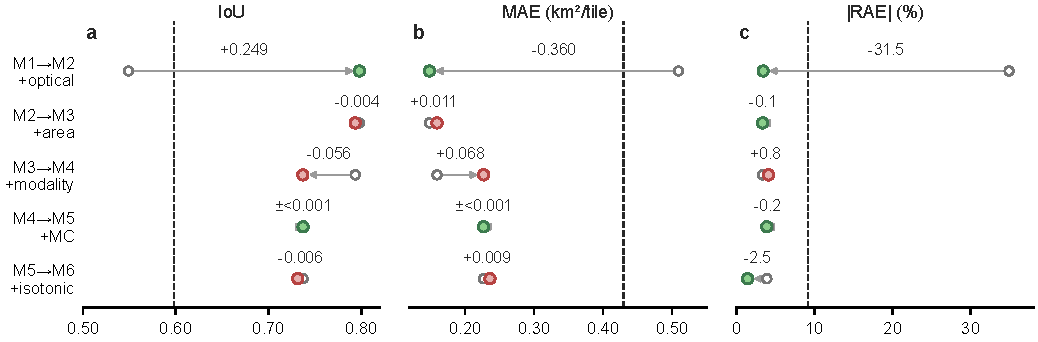
\includegraphics[width=0.90\textwidth,keepaspectratio]{../figures/fig_q2_ablation.pdf}
  \caption{Contribution of each component, M1 to M6}
  \label{fig:q2_ablation}
\end{figure}

Optical fusion is the decisive step: M1 to M2 raises IoU by 0.25 and cuts MAE$_A$ by 71\%. SAR-only M1 reaches IoU 0.549 and RAE $+34.9\%$, the measured cost of dropping the pre-flood land state, which alone separates a dark field or a permanent pond from new inundation; LightGBM paid no such cost because its features already contained NDWI. The area term changes little in-domain, modality dropout (a quarter of the training samples blinded) costs 0.06 IoU, and the MC mean leaves the metrics unchanged. Calibration cuts the total bias from $+4.1\%$ (M4) to $+1.45\%$: the tree stratum, $+74.87$\,km$^2$ of net error under LightGBM, contributes $-5.43$\,km$^2$ under M6, and the largest remaining nets are $+15.88$\,km$^2$ in wetland and $+15.20$\,km$^2$ in permanent water (Fig.~\ref{fig:q1_error_drivers}a).

Model choice was fixed before the test metrics were read: M2+MMU sets the in-domain ceiling at IoU 0.797, and M6 carries the SAR-only transfer because it pairs the calibrated area with a per-tile conformal interval, which is what Problem~3 consumes; its intervals cover the true tile area in 87.8\% of test tiles (folds 82.7--92.6\%, flood-share terciles 85.3--92.8\%) at a mean width of 0.54\,km$^2$.

\subsection{Data-Based Four-Level Intensity Grading}

Grading rests on the newly inundated area and its share of the study region, with explicit area or proportion thresholds. Because $\rho=A_{new}/A_{reg}$ is free of scale, thresholds are set on it and then translated into area thresholds for any unit:
\begin{equation}
A^*_g(A_{reg})=\theta_g\,A_{reg},\qquad g=1,2,3,
\label{eq:area_thr}
\end{equation}
with grade general for $\rho<\theta_1$, relatively strong for $\theta_1\le\rho<\theta_2$, strong for $\theta_2\le\rho<\theta_3$ and extremely strong for $\rho\ge\theta_3$. Round numbers are the wrong source for these cuts. The flood share of the 985 non-empty official tiles is strongly skewed; the fit is made on $x_t=\operatorname{logit}\rho^{ref}_t$ (with $\rho$ clipped to $[10^{-4},1-10^{-4}]$), a four-component Gaussian mixture by EM with 20 initializations. Adjacent components meet at their Bayes boundary, the root in $(\mu_g,\mu_{g+1})$ of
\begin{equation}
\pi_g\,\phi(x;\mu_g,s_g^2)=\pi_{g+1}\,\phi(x;\mu_{g+1},s_{g+1}^2),\qquad \theta_g=\frac{1}{1+e^{-x^*_g}},
\label{eq:gmm_bayes}
\end{equation}
where $\pi_g$, $\mu_g$, $s_g$ are the mixture weight, mean and standard deviation of component $g$ and $\phi$ the normal density. A tile sitting on the boundary is equally likely under both components, and the rule assigns it to the regime that most probably produced it. Fitted logit means are $-4.30$, $-1.85$, $1.24$ and $5.43$ with weights 0.544, 0.301, 0.098 and 0.057, which gives
\begin{equation}
\theta=(\theta_1,\theta_2,\theta_3)=(0.0593,\ 0.530,\ 0.969).
\label{eq:theta_values}
\end{equation}
Table~\ref{tab:grade_thr} translates them by \eqref{eq:area_thr} for three unit sizes.

\begin{table}[!ht]
\centering
\caption{Proportion and area thresholds of the four grades}
\label{tab:grade_thr}
\begin{tabular}{lcccc}
\toprule
Grade & $\rho$ range & Official tile 4.92\,km$^2$ & 1\,km$^2$ cell & Hengzhou 3440.4\,km$^2$ \\
\midrule
General & $<5.9\%$ & $<0.29$ & $<0.059$ & $<203.9$ \\
Relatively strong & 5.9--53.0\% & 0.29--2.61 & 0.059--0.530 & 203.9--1822.5 \\
Strong & 53.0--96.9\% & 2.61--4.77 & 0.530--0.969 & 1822.5--3333.5 \\
Extremely strong & $\ge96.9\%$ & $\ge4.77$ & $\ge0.969$ & $\ge3333.5$ \\
\bottomrule
\end{tabular}
\end{table}

How stable are these thresholds? We refit \eqref{eq:gmm_bayes} on 1000 block-bootstrap resamples of the 67 blocks. The 90\% intervals are $[0.0075,0.079]$ for $\theta_1$, $[0.067,0.655]$ for $\theta_2$ and $[0.522,0.998]$ for $\theta_3$, and 71\% of the resamples give a valid ordered four-component solution. The middle threshold is the least determined. BIC is lowest for two components (4604.8 against 4629.5 for four); the data alone do not demand four modes. Four grades are required by the problem, and the mixture is the most data-faithful way to place them. Jenks natural breaks on $x_t$ give $(0.035,0.371,0.967)$, close to the mixture for $\theta_1$ and $\theta_3$. The reference grades of the 1000 tiles are 575 general, 283 relatively strong, 89 strong and 53 extremely strong.

\subsection{How Area Errors Move the Grades}

A grade computed from an estimated area inherits its error. For unit $j$ we draw $m=1,\dots,M$ with $M=2000$ a residual $r^{(m)}$ from the pool $\mathcal R$ and a threshold vector $\theta^{(m)}$ from the bootstrap set:
\begin{equation}
\begin{split}
A_j^{(m)}&=\mathrm{clip}\big(\hat A_j+r^{(m)}\sigma'_j,\ 0,\ A_{reg,j}\big),\\
\pi_{jg}&=\frac1M\sum_{m=1}^M\mathbb 1\Big[G\big(A^{(m)}_j/A_{reg,j};\theta^{(m)}\big)=g\Big],\qquad
\sum_g\pi_{jg}=1,
\end{split}
\label{eq:grade_mc}
\end{equation}
where $G(\rho;\theta)$ is the grade of \eqref{eq:area_thr}. The vector $\pi_j$ replaces a single grade by a distribution that includes both the area error and the threshold uncertainty. Fig.~\ref{fig:q2_grading} shows the mixture fit and the resulting grade confusion.

\begin{figure}[t]
  \centering
  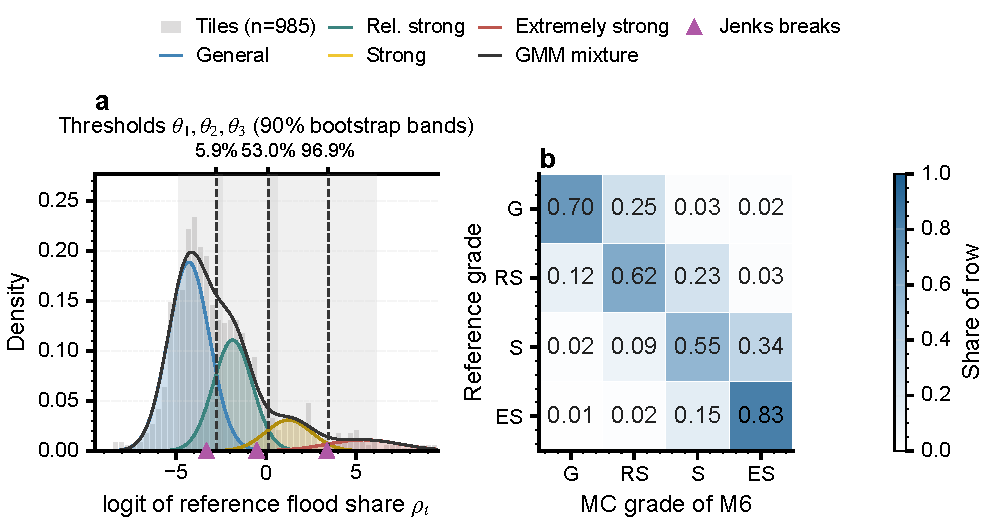
\includegraphics[width=0.90\textwidth,keepaspectratio]{../figures/fig_q2_grading.pdf}
  \caption{Gaussian-mixture grading and MC confusion}
  \label{fig:q2_grading}
\end{figure}

Where the two weakest regimes meet on the logit axis, the bootstrap bands of $\theta_1$ and $\theta_3$ stay narrow while that of $\theta_2$ widens (panel A). Row-normalized confusion against the Monte Carlo grade of M6 (panel B) keeps 70\% of the general, 62\% of the relatively strong, 55\% of the strong and 83\% of the extremely strong tiles in their grade, and the errors fall almost entirely into the neighboring grade. With the deterministic M6 area the grade is correct for 86.2\% of the tiles, against 54.3\% for LightGBM, so area calibration pays off directly in the grading. The expected Monte Carlo accuracy is 67.0\%, which prices in threshold uncertainty. Within four standardized errors of a threshold the flip probability $1-\max_g\pi_{jg}$ is 0.33--0.37, and 0.22 farther away; a unit near a threshold should therefore carry $\pi_j$ with its grade\cite{deepseek2026,qwen2026,doubao2026}.

Under a normal approximation of the signed tile-area error, Fig.~\ref{fig:q2_flip} makes the geometry explicit. Deep inside a grade the change probability is near zero; it peaks at one half exactly on a threshold, and the ridge widens with $\sigma$. Placing the 1000 test tiles in four bins at their mean estimated proportion and the standard deviation of their signed error gives $(1.1\%,0.026)$, $(10.2\%,0.098)$, $(32.1\%,0.141)$ and $(86.8\%,0.294)$. Two of the bins, the 5--20\% one and the highest, sit in the high-probability band of the surface -- consistent with the Monte Carlo flip rate of 0.33--0.37, even though most tiles lie far from $\theta_2$ and $\theta_3$.

\begin{figure}[!ht]
  \centering
  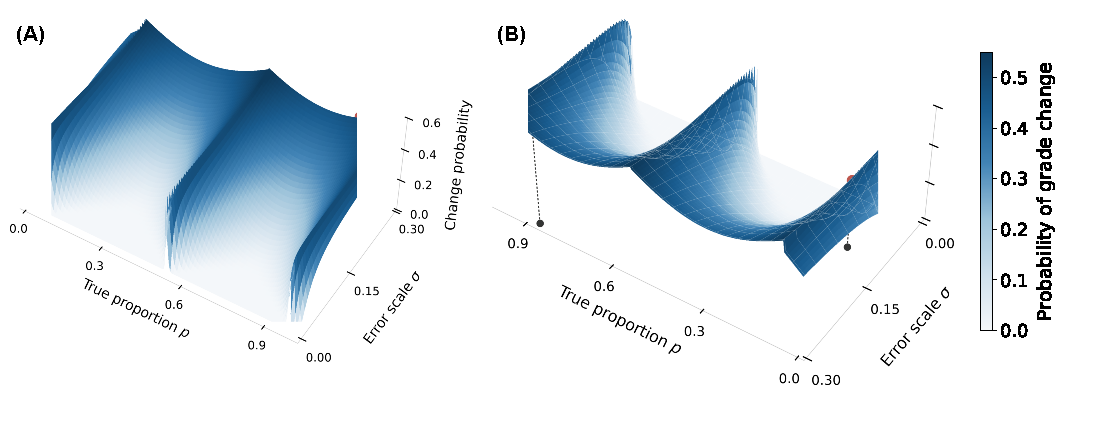
\includegraphics[width=0.90\textwidth,keepaspectratio]{../figures/fig_q2_flip_surface.pdf}
  \caption{Grade-change probability surface}
  \label{fig:q2_flip}
\end{figure}
